\documentclass{article}
\usepackage[utf8]{inputenc}
\usepackage[german]{babel}
\usepackage[legalpaper, portrait, margin=1in]{geometry}
\usepackage{setspace}
\onehalfspacing
\usepackage{parskip}
\setlength{\parindent}{0cm}
\usepackage{enumitem}
\setlist{nosep}
\usepackage{hyperref}
\usepackage{graphicx}

\hypersetup{
  	colorlinks,
	citecolor=black,
	filecolor=black,
	linkcolor=black,
	urlcolor=black
}
\title{%
  Olympus DAO Manifesto \\
  \large Funktionales DAO für Open-Source Kryptowährung Projekte.}
\author{
  Berrueta, Enrique\\
  \texttt{eabz@polispay.org}
  \and
  Bustos, Ricardo\\
  \texttt{eros@polispay.org}
}
\date{Juni 2020}

\begin{document}

\maketitle

	\begin{abstract}
    Eine DAO ist eine ``Dezentralisierte Autonome Organisation`` oder eine Körperschaft ohne zentrale Autorität, die von einer Mehrparteien-Organisation autorisierter Mitglieder regiert werden kann, die von einer größeren Gemeinschaft ausgewählt werden. Im Laufe der Jahre wurden seit Beginn der Kryptowährungen mehrere DAO- und Regierungsversuche unternommen. Von Dash bis zu Ethereums ``The DAO`` hatten all diese Organisationen verschiedene Probleme, von mangelnder Organisation bis zur völligen Zentralisierung. Nachdem ich darüber nachgedacht habe, bin ich gekommen, um eine neue Lösung für die Schaffung einer funktionalen DAO vorzuschlagen, die nicht nur dezentralisiert, sondern auch organisiert und inklusiv sein wird.
	\end{abstract}

\newpage

\tableofcontents


\newpage

\section{Struktur}

Die DAO wird sich auf fünf Grundsäulen stützen, von denen es für jede Säule einen von der Gemeinschaft gewählten Verantwortlichen geben wird:

\begin{itemize}
  \item Technologie.
  \item Gemeinschaft.
  \item Geschäft.
  \item Übernahme.
  \item Marketing.
\end{itemize}

\begin{figure}[h]
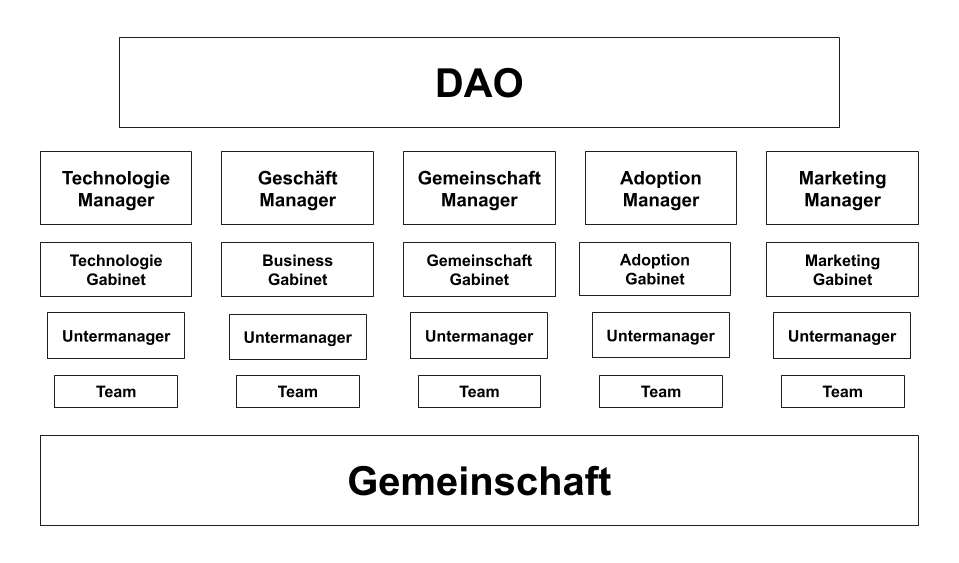
\includegraphics[scale=0.4]{img/dao_structure_de.png}
\centering
\caption{Grundlegendes Organisationsmodell der DAO}
\end{figure}

Jede verantwortliche Person, die von nun an als ``Manager`` bezeichnet wird, ist aufgrund ihres Prestiges in der Gemeinschaft wählbar. Sie werden der Gemeinde einen Vorschlag vorlegen, in dem sie ihre Vorschläge für den Befehlszyklus detailliert darlegen, der ein Jahr dauern wird.

Auf ihren Vorschlag muss jeder Manager die folgenden Punkte beschreiben:

\begin{itemize}
  \item Verbesserungsvorschläge.
  \item Mitglieder ihres Teams (Kabinett).
  \item Strategien, die sie anwenden werden, um ihre Vorschläge zu verwirklichen.
  \item Warum sollte die Gemeinschaft für sie stimmen?
  \item Detaillierter Fahrplan mit spezifischen Zeitplänen eingeführt.
\end{itemize}

Die Manager können so oft wiedergewählt werden, wie sie es wünschen, solange die Gemeinschaft mit ihnen zustimmt.

\section{Schlüssel}

Da die gesamte DAO als ein Kryptowährungs-Ökosystem bezeichnet wird, sollte alles, was mit Abstimmungen und Entscheidungsfindung zu tun hat, mit einem DAO-Schlüssel erfolgen. Diese Schlüssel werden vom Manager gesichert und der Zugang wird während der DAO-Abstimmungszyklen oder der Ausführung eines Sicherheitsmechanismus gewährt/entfernt.

Diese Schlüssel werden im Laufe der DAO-Zyklen geändert, wenn sich die Position eines Managers in einem Abstimmungszyklus oder bei einem Sicherheitsmechanismus ändert. Dieser Schlüssel ist der Münzempfänger für das spezifische Gebiet und wird verwendet, um die Münzen (zusammen mit den anderen 5 Managern) für die Vorschläge der Gemeinschaft und den Überbudget zu entsperren.

\section{Plattform}

Die Plattform, um zu interagieren, abzustimmen, der DAO Vorschläge zu unterbreiten, ist die Olympus Blockchain.

Jeder Benutzer ist in der Lage, die Informationen der DAO in Echtzeit zu überprüfen, verifiziert durch einen vollständigen Knoten. 

Die Brieftasche von Olympus ist die Hauptplattform, die die Benutzer täglich für die Funktionen der DAO nutzen sollten.

\section{Treasury}

Damit eine DAO als Organisation ordnungsgemäß arbeiten kann, muss sie unbedingt über Fonds verfügen. Da es nicht möglich ist, sie auf der Grundlage von Spenden zu unterstützen, schlagen wir hier ein Finanzierungsmodell vor, das eine gerechte Finanzierung und ein Verteilungsmodell für jedes Gebiet garantiert.

Die 20\% der monatlich ausgegebenen Münzen werden auf ein Konto gesperrt, das für die DAO verwendet wird.

Diese Fonds werden in drei Kategorien verteilt:

\begin{itemize}
  \item 10\% zu den DAO-Gebieten.
  \item 5\% für Gemeinschaftsvorschläge.
  \item 5\% gesperrt für Gebiete, die das Budget überschreiten.
\end{itemize}

Das Budget für die DAO-Gebiete wird nach folgenden Proportionen verteilt:

\begin{itemize}
  \item 30\% Technologie.
  \item 10\% Gemeinschaft.
  \item 20\% Geschäft.
  \item 20\% Marketing.
  \item 20\% Übernahme.
\end{itemize}

Die 5\% für Gemeinschaftsvorschläge sollten auf der Grundlage der Entscheidung des Managers verteilt werden. Sie werden entscheiden, wann ein Vorschlag finanziert werden sollte.

Die 5\% für Gebiete, die das Budget überschreiten, sollten auf der Grundlage der Entscheidung des Managers verwendet werden, das Budget eines bestimmten Gebiets für einen bestimmten Zeitraum zu erhöhen.

Die Fonds werden jeden Monat vom Netzwerk automatisch an den aktuellen Manager Schlüssel eingezahlt.

Die über dem Budget liegenden Beträge der Gemeinschaft und der Gebiete werden auf einen mit mehreren Unterschriften versehenen Schlüssel eingezahlt, um sicherzustellen, dass nur 3 von 5 Managern in der Lage sind, diese Fonds abzuheben.

Die Vorschläge der Gemeinschaft müssen detailliert sein:

\begin{itemize}
  \item Höhe des erforderlichen Budgets.
  \item Aktionsplan
  \item Detailliertes Kostenbudget.
\end{itemize}

\section{Zyklen}

Die Funktionalität der DAO wird durch Zeitzyklen bestimmt. Es gibt nur drei Zyklen, die Entscheidungen zu verschiedenen Zeitpunkten beinhalten.

\subsection{Wahlzyklus}

Der Wahlzyklus beginnt jedes Jahr am 20. Januar. Dieser Prozess dauert etwa 2 oder 3 Wochen, und die Idee ist es, eine Wahlkampagne durchzuführen, bei der alte Manager und neue Mitglieder, die sich technisch in der DAO engagieren wollen, ihre Vorschläge und Fahrpläne machen müssen, um sich zu qualifizieren.

Dieser Zyklus besteht aus vier Phasen:

\begin{itemize}
  \item Kandidaten Postulate.
  \item Kandidaten Vorschläge.
  \item Wahlvorbereitungen.
  \item Abstimmung.
\end{itemize}

\subsection{Budgetierungszyklus}

Sobald die Manager ausgewählt sind, müssen sie ein ordentliches Budget vorlegen, mit dem sie die nächsten drei Monate arbeiten werden. Dieses Budget sollte vom Geschäftsführer alle drei Monate einschließlich des Budgets und der tatsächlichen Ausgaben vorgelegt werden, um die Gemeinschaft mit transparenten Informationen zu versorgen.

\subsection{Berichtszyklus}

Neben den Budgetzyklen sollte jeder Manager in seinen eigenen Gebieten einen Bericht über die Erfolge der 3-monatigen Arbeit für die Manager und die Gemeinschaft erstellen.

Wenn ein Manager den Bericht nicht in das Netzwerk hochlädt, wird sein Schlüssel automatisch aus den DAO-Schlüsseln entfernt.

\section{Gebiete}

\subsection{Technologie}

Der für Technologie zuständige Manager wird für die Einstellung und Ausbildung von Entwicklern verantwortlich sein, die den technischen Fahrplan der DAO befolgen.

Der Manager wird die folgenden Pflichten haben:

\begin{itemize}
  \item Kryptowährungstechnologie Entwicklung.
  \item Anwendungsfälle Entwicklung.
  \item Drittbibliotheken.
  \item Dokumentation und Wartung.
\end{itemize}

Daneben ist der Gemeinschaftsmanager für die ordnungsgemäße Funktionalität und Dokumentation der folgenden Dienste zuständig:

\begin{itemize}
  \item Offizielle Blockforscher.
  \item Webseiten.
  \item Leitfaden.
  \item Foren.
  \item Interne Ressourcen.
\end{itemize}

\subsection{Gemeinschaft}

Der für die Gemeinschaft verantwortliche Manager ist für die Gemeinschaft und die Integrität und Richtigkeit der auf den verschiedenen Kanälen angezeigten Informationen verantwortlich.

Der Manager hat die folgenden Pflichten:

\begin{itemize}
  \item Kommunikation und soziale Medien.
  \item Dokumentation und Wartung.
  \item Technischer Support für Benutzer und beste Sicherheitsverfahren.
  \item Korrektes Branding und Design.
\end{itemize}

Daneben ist der Technologiemanager für die ordnungsgemäße Funktionalität und Dokumentation der folgenden Dienstleistungen zuständig:

\begin{itemize}
  \item Offizielle Blockforscher.
  \item Webseiten.
  \item Leitfaden.
  \item Foren.
  \item Interne Ressourcen.
\end{itemize}


\subsection{Geschäft}

Der für die Geschäfte verantwortliche Manager ist dafür verantwortlich, neue Partnerschaften mit anderen Projekten aufzubauen und die Vorschläge der Gemeinschaft zu verfolgen.

Der Manager hat die folgenden Pflichten:

\begin{itemize}
  \item Partnerschaften.
  \item Verwaltung und Budgettransparenz.
  \item Vorschläge der Gemeinschaft werden weiterverfolgt.
\end{itemize}

\subsection{Übernahme}

Der für die Übernahme verantwortliche Manager wird dafür verantwortlich sein, Händler in das Projekt einzubinden und neue Entwickler dazu zu bringen, die Technologie für ihre Zwecke zu nutzen und Veranstaltungen zu organisieren, um die Nutzung des Netzwerks anzuziehen.

Der Manager wird die folgenden Pflichten haben:

\begin{itemize}
  \item Händler Übernahme.
  \item Entwickler Übernahme.
  \item Büro für Öffentlichkeitsarbeit und Information.
\end{itemize}

\subsection{Marketing}

Der für das Marketing verantwortliche Manager wird für die Suche nach geeigneten Räumen zuständig sein, solange er die anderen Manager mit analytischen und Marketing-Strategien versorgt.

Der Manager hat die folgenden Pflichten:

\begin{itemize}
  \item Marketingstrategien, Linien und Fahrpläne.
  \item Analyse- und Informationsberichte.
  \item Werbeflächen.
\end{itemize}

\section{Sicherheitsmechanismus}

Da die DAO das Vertrauen der bekannten Mitglieder in die Organisation voraussetzt, sollten Sicherheitsmechanismen entwickelt werden, die auf der Diskussion und der Sicherheit des Netzwerks basieren.

Wir sahen nur zwei mögliche Fälle vor, in denen ein Problem mit der Struktur oder den Mitteln der DAO auftreten kann. Um diese Fälle abzudecken, bauten wir den folgenden Sicherheitsmechanismus auf.

\subsection{Manager Sperrung}

Wenn die Manager unter irgendwelchen Umständen ein Mitglied entfernen möchten, können sie ihren DAO-Schlüssel verwenden, um eine signierte Nachricht an das Netzwerk für die Entfernung des Schlüssels aus den DAO-Schlüsseln zu erstellen. Damit dieser Mechanismus ausgeführt werden kann, benötigt er mindestens 3 von 5 möglichen Signaturen.

\subsection{DAO Sperrung}

Dieser Mechanismus wird von der Gemeinschaft ausgeführt, er impliziert, dass die Manager auf irgendeine Weise ihre Arbeit nicht korrekt ausführen oder die gesamte DAO von einer Gruppe übernommen wird, die dem gesamten Ökosystem schadet.

Die Mitglieder der Gemeinschaft können eine unterschriebene Nachricht mit dem Nachweis des Besitzes einer Anzahl von Münzen erstellen. Sobald die Schwelle von 30\% des gesamten Münzvorrats überschritten ist, werden alle Schlüssel der DAO entfernt und ein Notabstimmungszyklus beginnt.

\end{document}
